%%% Local Variables:
%%% mode: latex
%%% TeX-master: t
%%% End:

\documentclass[master, openany, oneside]{tongjithesis}
%开始用了openright,但这样即每章都是奇数页开始,但实际上,只需要摘要、目录、英文摘要、正文第一章、
%参考文献、附录、个人简历都从奇数页开始即可,正文内部章节可以从偶数页开始,因此用\cleardoublepage命令实现

% \documentclass[%
%   master|doctor, % mandatory option
%   xetex|pdftex|dvips|dvipdfm, % optional
%   secret,
%   openany|openright,
%   arialtoc,arialtitle]{tongjithesis}

% 所有其它可能用到的包都统一放到这里了,可以根据自己的实际添加或者删除。
\usepackage{tongjiutils}
\usepackage[top=1.3in,bottom=1.15in,left=1.25in,right=1.25in]{geometry}%调节每一页的页面大小,
\usepackage[figuresright]{rotating}
\usepackage{graphicx}
\usepackage{titlesec}
\usepackage{algorithmicx}
\usepackage{algpseudocode}
\usepackage{etex}
\usepackage[perpage,symbol*,bottom]{footmisc} %使用了\raggedbottom后仍然保持脚注在页面底部,且脚注在每一页都从1开始,
%符合规范,脚注形式为①,另外,此命令与下面命令还可以使得模板原先的自动填充的空白得到很好的控制,如果没有这个命令,
%章节标题与正文间的空白很难控制,特别是有图、表与公式的时候
\raggedbottom
\usepackage{epstopdf}
\usepackage{fancyhdr}
\usepackage{verbatim}
\usepackage{CJKpunct}
\usepackage{setspace}
\usepackage{longtable}
\usepackage{url}
\usepackage{pifont}
\usepackage{algorithm}
\usepackage{ulem}
\usepackage{extarrows}
\usepackage{caption}
\setlength\parskip{0pt}
\frenchspacing
\widowpenalty=10000
%此命令貌似是用来修改图标与正文的间距的


% 你可以在这里修改配置文件中的定义,导言区可以使用中文。
\def\myname{同济人}

\begin{document}

% 定义所有的eps文件在 figures 子目录下
\graphicspath{{figures/}}


%%% 封面部分
\frontmatter

%%% Local Variables:
%%% mode: latex
%%% TeX-master: t
%%% End:
%\secretlevel{保密} \secretyear{2}

\ctitle{基于图像的轻量化3D树木建模方法\\ [2ex] \begin{large} \raisebox{0.5mm}{------}PyrLK光流法树木重建解决方案的增强与优化 \end{large}}

% 按照申请工学学位设计。如有其它需要,请修改相应文字。
\makeatletter
  \iftongji@doctor
    \cdegree{工学博士}
  \else
    \iftongji@master
      \cdegree{毕业设计(论文)}
    \fi
  \fi

\makeatother

\cdepartment{软件学院}

\cmajorfirst{软件工程}

\cmajorsecond{软件工程}

\cauthor{张德嘉}

\snumber{092792}

\csupervisor{贾金原}

% 如果没有副指导老师或者联合指导老师,把各自{}中内容留空即可。

\cassosupervisor{}

\ccosupervisor{}

% 定义中英文摘要和关键字
\begin{cabstract}
随着当今WebVR、WebGame、WebGIS等基于Web的应用迅猛发展,为了适应网络传输以及用户日益增长的对图形效果的追求,真实感与轻量化
之间的矛盾日益激化。为了解决这个矛盾,本课题提出了一套高效、低成本的分级轻量化树木建模方法。它以改进的三维重建算法为基础,
进行基于用户交互地自动化骨架抽取,并根据应用需求,可进行分级的轻量化。这种分级轻量化方法可以进一步被扩展为自适应网络带宽
或用户硬件条件的树木模型生成方法。

为了实现高效的分级轻量化建模方法,本文首先将PyrLK光流法进行基于仿射变换和反向追踪的改进,并且将其运用到三维重建
的特征点匹配步骤中,以提高树木特征点的匹配率和稳定性。然后进行GPU加速的三维重建以得到高精度点云模型。接着本文
运用三维体素泛洪和最小二乘线性拟合的方法对树木骨架和半径信息进行抽取,以适应树木生长规律的方法抽取出了准确的骨架。
对于算法的主观性和可能造成的二义性,本文又提出了基于用户指引的算法补全措施,以进一步提高建模的准确性和鲁棒性。
然后本文提出了根据应用对轻量化的需求等级,对骨架进行纵向和横向的合并,以减小骨架的尺寸来实现轻量化,从而更好地适应
面向网络的应用的需求。最后本文还给出了一套完整的基于图像树木建模的质量评价,提出了还原度的概念来客观、量化地评价建模出
的模型的还原度以及在轻量化过程中质量的丢失。
\end{cabstract}

\ckeywords{基于图像三维重建, 树木建模, 轻量化模型,PyrLK光流法,骨架抽取}

\begin{eabstract}
As the Web-oriented applications(WebVR, WebGame,
WebGIS, etc) develop rapidly and the persuit of graphics effect boosts quickly, the lightweight and realism of tree modeling are badly
needed nowadays. In order to solve the contradiction between lightweight and realism, this article proposes a high-efficiency、low-cost and
multi-level lightweight tree modeling method. Based on the improved 3D reconstruction methods, it conducts a user-sketch automatic skeleton 
extraction. And it uses multi-level lightweight method to meet the applications' needs, which can be improved to automatically fit the 
bandwidth and hardware conditions of the client side.

For implementing the lightweight method, we first improve the traditional PyrLK optical flow method to support affine transformation
and backward feature tracking, which can furthur be applied to do feature matching in gpu accelerated 3D reconstruction and 
improve the match ratio. Then we use flooding algorithm in 3D voxel model and least squares method to discover the tree skeleton and
its radius information. In order to improve the accuracy and robustness of the algorithms, this article suggests a few use sketches.
And according to the lightweight level the applications require, we reduce the model size by merging the
branches vertically and horizontally respectively. At last we propose a modeling quality evaluation method, which will objectively and 
quantizedly evaluate the restore degree of the tree model.
\end{eabstract}

\ekeywords{Image-based 3D Reconstrction, Tree Modeling, Light-weight Modeling, PyrLK Optical Flow, Skeleton Extraction}

\makecover


% 目录

\tableofcontents

% 符号对照表
%\begin{denotation}
\item[GNU] GNU's Not Unix /'gnu:/
\item[GFDL] GNU Free Documentation License
\item[GPL] GNU General Public License
\item[FSF] Free Software Foundation
\item[SMP] 对称多处理
\item[API] 应用程序编程接口
\item[$E$] 能量
\item[$m$] 质量
\item[$c$] 光速
\item[$P$] 概率
\item[$T$] 时间
\item[$v$] 速度
\end{denotation}


%%% 以下索引按需要选择
% 插图索引
%\listoffigures
% 表格索引
%\listoftables
% 公式索引
%\listofequations

%%% 正文
\mainmatter
\include{data/chap01}
\include{data/chap02}
\include{data/chap03}

\chapter{Improved PyrLK Optical Flow Method}
\label{cha:pyrlk}
%----------------------------------PyrLK--------------------------------------
The first step of image-based tree modeling is 3D reconstruction, and the first
step of 3D reconstruction is character matching, which is to find a same space 
point projecting onto 2 frames. This article chooses Harris corners as the character
points, which can be affine invariant. The traditional PyrLK optical flow is rather 
limited, because:\\

\begin{itemize}
	\item \textbf{No Rotation Support} The traditional PyrLK optical flow method doesn't support
		rotation of character points, which will certainly limit its extension.
	\item \textbf{Lack Validation Methods} The traditional PyrLK lacks validation methods, which will
		lead to too many match errors, and will no doubt cause more trouble to the subsequent 3D 
		reconstruction steps.
\end{itemize}

In order to solve these two problems, this article proposes an affine transformation and back track based
PyrLK optical flow method, which can give a solution to the problems above, and ensure the robustness and 
correctness of the 3D reconstruction.

%\subsection{对于SIFT特征点匹配的尝试}
%对于特征点的匹配,本文首先尝试的是利用VisualSFM工具自带的SIFT特征点匹配。
%但是经过大量实验发现,该工具自带的SIFT特征点匹配并不能很完整地找到匹配的
%点对,从而导致了三维重建所依赖的数据不足、不精确,最后重建出来一个缺失度
%很大的模型,这样的模型显然不能成功的进行骨架抽取。
%
%根据实验结果分析,除开

\section{Optical Flow Introduction}
The concept of optical flow is proposed by James Gibson. 1981, Horn and Schunck connect the 
2D velocity field with the gray scale creatively and provided an effective calculation method
for optical flow\cite{horn}. They assume the light intensity stay invariant, and the grayscale
of the image changes as the background or target moves. Under such assumption, the optical flow
method detects the target motion through different velocity of target and background.

Moreover, when the objects in 3D scene move against the 2D image plane, the projection on 2D image
plane forms the motion, which turns out to be optical flow when it is represented in the grayscale mode.
In other words, the optical flow is the immediate velocity of the object on the view plane, which is 
measured by the displacement of pixels in the image. The optical flow filed is the set of optical flow
point and is a 2D immediate velocity field. It can represent the displacement of the whole image, which
can be used to detect the motion of 3D targets.

After optical flow method was proposed, many scholars have studied on it and improved it. Each method has
its advantages, and the efficiency and applications vary. One of the most typical one is the Lucas-Kanade
local smooth method(LK optical flow)\cite{lk}, which uses differential of time and space to calculate the 
speed vector and smooth out the image to track the optical flow. And in 2000, Jean-Yves proposed a pyramidial
implementation of LK optical flow method, which is called PyrLK optical flow method\cite{pyrlk}.

\section{PyrLK Optical Flow method}
\label{subsec:pyrlk}
Assume the value function of pixels is $I(x,y,t)$,which indicates the value of pixel on $(x,y)$ is $I(x,y,t)$
at time $t$. So after $\Delta t$,the pixel value will change to $I(x+\Delta x,y+\Delta y, t+\Delta t)$。
Here is the reduction:\\
\[  I(x+\Delta x,y+\Delta y, t+\Delta t)=I(x,y,t) + \frac{\partial I}{\partial x}\Delta x 
		+ \frac{\partial I}{\partial y}\Delta y + \frac{\partial I}{\partial t}\Delta t \]
\begin{displaymath}
	\begin{array}{cc}
		\implies & \frac{\partial I}{\partial x}\Delta x 
		+ \frac{\partial I}{\partial y}\Delta y + \frac{\partial I}{\partial t}\Delta t = 0\\
		\implies & \frac{\partial I}{\partial x}V_x 
		+ \frac{\partial I}{\partial y}V_y + \frac{\partial I}{\partial t} = 0 
	\end{array}
\end{displaymath}
\begin{equation}\label{eq:opticalflow}
	\begin{array}{cc}
				\implies & I_xV_x + I_yV_y = -I_t
	\end{array}
\end{equation}

Lucas-Kanade Optical Flow is based on principles above, and it assumes that the displacement between
two frames is small, and it stays constant in a neighborhood region. Under such assumptions, an equation
set can be listed: \\
\begin{equation}
	\left\{
		\begin{array}{c}
			I_x(q_1)V_x + I_y(q_1)V_y = -I_t(q_1)\\
			I_x(q_2)V_x + I_y(q_2)V_y = -I_t(q_2)\\
			\vdots\\
			I_x(q_n)V_x + I_y(q_n)V_y = -I_t(q_n)\\
		\end{array}
	\right.
\end{equation}

The $q_1,q_2,...,q_n$ is the points in local window,And $I_x(q_i),I_y(q_i),I_z(q_i)$ is the partial derivative
at $q_i$ of image $I$ in direction $x,y,t$, which can be written in matrix form:
\begin{equation}
	A=	
	\left(
	\begin{array}{cc}
		I_x(q_1) & I_y(q_1)\\
		I_x(q_2) & I_y(q_2)\\
		  \vdots & \vdots\\
		I_x(q_n) & I_y(q_n)
		\end{array}
	\right),\quad
	v=
	\left(
	\begin{array}{c}
		V_x\\
		V_y
	\end{array}
	\right),\quad
	b=
	\left(
	\begin{array}{c}
		-I_t(q_1)\\
		-I_t(q_2)\\
		\vdots\\
		-I_t(q_n)
	\end{array}
	\right)
\end{equation}

The number of unknowns is far greater than the number of equations, so $A$ is over determined, LK optical flow
uses the least squares method to calculate the optical flow velocity. 

Although the LK optical flow method is intuitive, there is a problem. The motion block detected is positive correlation,
so in order to catch the motion of big block, it's supposed to largen the size of window. But as the size of window increases,
the velocity should keep stable in a larger region, which is against the assumption of the method. The pyramidial implementation
of Lucas-Kanada method solves this problem, and its ideas are given below:\\

Assume $I$ and $J$ are two grayscale images,$I(x)$ and $J(x)$ is the grayscale value at $(x,y)$ in $I$ and $J$。Consider a point
$\mathbf{u}=(u_x, u_y)$ on image $I$,The goal of character tracking is to find a corresponding point $\mathbf{v}
=\mathbf{u}+\mathbf{d}=(u_x+d_x,u_y+d_y)$ on J,which makes that $I(\mathbf{u})$ and $J(\mathbf{v})$ are similar。Vector
$\mathbf{d}=(d_x,d_y)$ is the optical flow velocity at point $\mathbf{x}$。Then the similarity of the neighborhood is defined,
assume $\omega_x$ and $\omega_y$ are two integers,the velocity is the vector $\mathbf{d}$ which lets the formula reach its minimum:\\
\begin{equation}\label{eq:similarity}
	\epsilon(\mathbf{d})=\epsilon(d_x,d_y)=\sum_{x=u_x-\omega_x}^{u_x+\omega_x}\sum_{y=u_y-\omega_y}
	^{u_y+\omega_y}(I(x,y) - J(x+d_x,y+d_y))^2.
\end{equation}
The size of neighbor window is $(2\omega_x+1)\times(2\omega_y+1)$。This formula indicates to find a vector $\mathbf{d}$
letting the difference of $\mathbf{u}$ and $\mathbf{v}$ reach minimum in neighborhood region。

Then this method uses the pyramidial representation of image, which uses the source image as the highest resolution level,
and iteratively downsamples the image, one new resolution level can be got after each iteration. By doing this, the constant
window size can map to a larger area in low resolution image, and the big block motion is supported then.

\section{Improved PyrLK Optical Flow Method}
\label{subsec:revisedpyrlk}
\subsection{Support Affine Transformation}
The PyrLK optical flow method has already worked well on translation-oriented match. However, this is not the best way
to solve the matching problems on trees. Because the two adjacent frames are taken from two diffrent angles, so the character
points should have some transformation motion. However, this is not solved in traditional PyrLK method. Therefore, there is 
need to extend the method to support affine transformation.

Assume two points fit the affine matrix $A$,So:\\
\begin{equation}
	\left(
	\begin{array}{c}
		\Delta x'\\
		\Delta y'\\
		0
	\end{array}
	\right)
	=
	\left(
	\begin{array}{ccc}
		a_{11} & a_{12} & a_{13}\\
		a_{21} & a_{22} & a_{23}\\
				0 & 0 & 0
	\end{array}
	\right)
	\cdot
	\left(
	\begin{array}{c}
		\Delta x\\
		\Delta y\\
		1
	\end{array}
	\right)
\end{equation}
Take that to equation \ref{eq:opticalflow}:\\
\begin{equation}
	(a_{11}\ a_{12}\ a_{13}\ a_{21}\ a_{22}\ a_{23})\cdot
	\left(
	\begin{array}{c}
		\frac{\partial I}{\partial x}\Delta x\\
        \frac{\partial I}{\partial x}\Delta y\\
        \frac{\partial I}{\partial x}\\
        \frac{\partial I}{\partial y}\Delta x\\
        \frac{\partial I}{\partial y}\Delta y\\
        \frac{\partial I}{\partial y}\\
	\end{array}
	\right)
	=-I_t
\end{equation}

Matrix $A$ can be sovled by using the least squares method.

Modify the definition equation \ref{eq:similarity} to support the affine transformation:\\
\[ Let\quad \mathbf{a_1}=(a_{11},a_{12},a_{13})\quad \mathbf{a_2}=(a_{21},a_{22},a_{23})\quad
\mathbf{b}=(d_x,d_y,1)\]\\
\begin{equation}\label{eq:affine}
	\epsilon(\mathbf{d})=\epsilon(d_x,d_y)=\sum_{x=u_x-\omega_x}^{u_x+\omega_x}\sum_{y=u_y-\omega_y}
	^{u_y+\omega_y}(I(x,y) - J(x+\mathbf{a_1}\cdot \mathbf{b},y+\mathbf{a_2}\cdot \mathbf{b}))^2.
\end{equation}


\subsection{Back tracking and Median Filtering}
The several previous sections are discussing the extension stuff of the method. However, how can
we make sure the two matching points really match. The traditional PyrLK method hasn't solved this
problem, which makes it unreliable. The present method lacks bidirectional check, which means that
the similarity of two matching points should be bidirectional. So this article proposes the back
tracking method to validate this quality.

Moreover, any matching algorithm can't make promises that it's perfectly matching. So after finishing
the algorithm, it should drop some "edge" matches, which can make the result more robust. This article
proposes a median filtering method, which can filter out those whose similarity is below the median line:\\

\begin{itemize}
	\item \textbf{Neighborhood Similarity Median Filtering}: After the PyrLK is conducted, for each matching pair, 
		we compute their normalized correlation as their similarity。The formular is given below:\\
		\begin{equation} \label{eq:ccoeff}
			R(x,y) = \frac{\sum_{x',y'}(T'(x',y')\cdot I'(x + x', y + y'))}
			{\sqrt{\sum_{x', y'}T'(x',y')^2\cdot \sum_{x',y'}I'(x+x',y+y')^2}}
		\end{equation}
		And then compute the median value of all the similarity, for those less than this value, we drop them.
	\item \textbf{Back Tracking Error Median Filtering}: After we conduct the back tracking,each pair will get an error value,which indicates the
		space position difference between the back track point and the source point. This article will drop those less than the median error value.
\end{itemize}

The remaining points after back tracking and median filtering will be considered as the robust match result.
Algorithm \ref{alg:backtrack} gives the pseudo-code of back tracking and median filtering:\\
\begin{algorithm}[H]
	\caption{Back Tracking \& Median Filtering}
	\label{alg:backtrack}
	\begin{algorithmic}[1]
	\Require Back Tracking Error Array $\mathbb{B}[1..n]$,Neighborhood similarity array $\mathbb{S}[1..n]$
	\Require Source matching pair array $\mathbb{P}$
	\Ensure Desitination matching pair array $\mathbb{Q}$
	\State Initialize back tracking error median value $mid_{back}$,Neighborhood similarity median value $mid_{similar}$
	\State SortArray($\mathbb{B}[1..n]$)
	\State SortArray($\mathbb{S}[1..n]$)
	\State $mid=(n+1)/2$
	\State $mid_{back}=\mathbb{B}[mid],\quad mid_{similar}=\mathbb{S}[mid]$
	\For{$i=1$ to $n$}
	\If{$\mathbb{B}[i] < mid_{back} \cap \mathbb{S}[i] > mid_{similar}$}
		\State $\mathbb{Q}.AddMatch(\mathbb{P}[i])$
	\EndIf
	\EndFor
	\State \Return $\mathbb{Q}$
	\end{algorithmic}
\end{algorithm}

\section{PyrLK with Robustness Improvement and Affine Transformation Support}
The adaptability and stability are improved a lot after PyrLK supports the affine transformation
and improves the robustness, which results in:\\
\begin{itemize}
	\item \textbf{Support Rotation}: Each two frames are the projection of 3D Rotation, so the rotation
		support is important, since it happens on every pair. By doing so, the accuracy can be improved a lot.
	\item \textbf{Matching Validation}: For each matching pair, this article uses normalized correlation to 
		calculate their similarity. Only those who pass the similarity validation can be the real mathcing pairs.
	\item \textbf{Eliminate Matching Mistakes}: Matching in only one direction can be unreliable, so this article
		uses back tracking to do bidirectional validation, which can improve the robustness of the algorithm.
\end{itemize}

Figure\ref{fig:pyrlk} gives the contradiction between the improved version and the traditional version. The images here
use different color path to represent the two adjacent frames, where the green path represents the previous picture and 
the purple path represents the next picture, and the red line indicates the matching relationship. From figure\ref{fig:pyrlk}(a)
we can find, there are bunches of errors with the traditional method for its lack of validation. For example, the trees far away
from sight should be sensitive to the rotation of camera, but figure\ref{fig:pyrlk}(a) doesn't catch this. And there are lots of
points matching to the background incorrectly. In figure\ref{fig:pyrlk}(b), the optical flow is appropriate and doesn't have the 
problems just metioned. So the improved version has an appreciative effect.
\begin{figure}[H]
	\centering
	\subfloat[Traditional PyrLK]{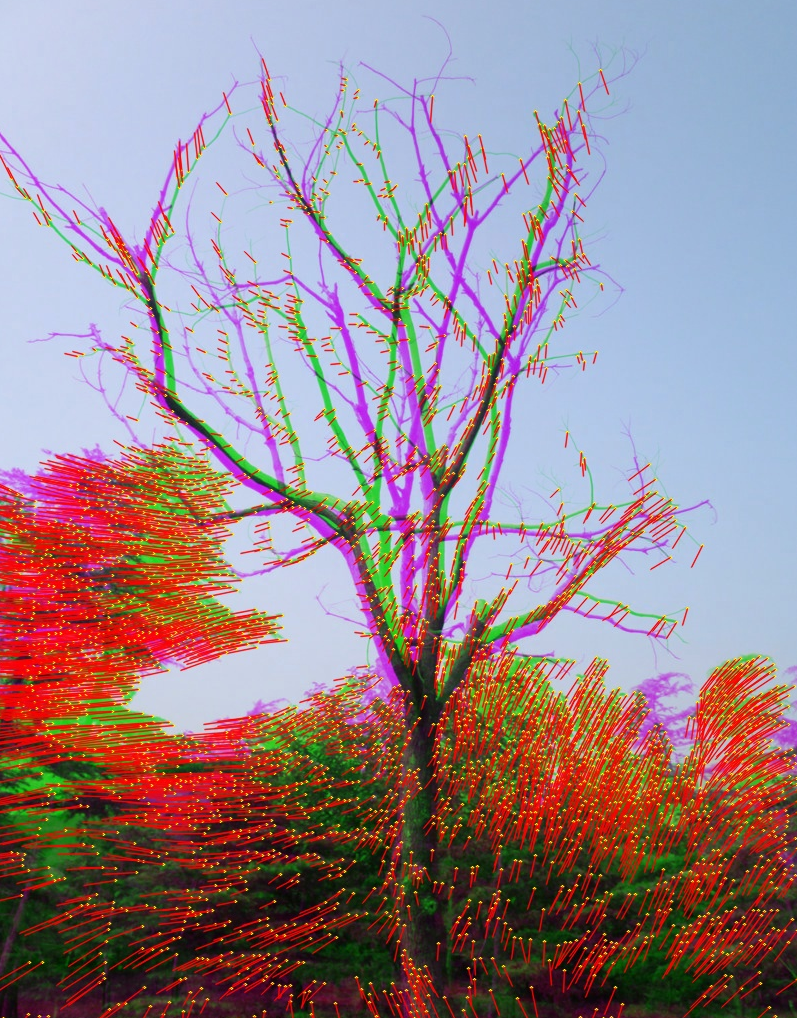
\includegraphics[height=10cm]{old.png}}\hspace{4em}
	\subfloat[Improved PyrLK]{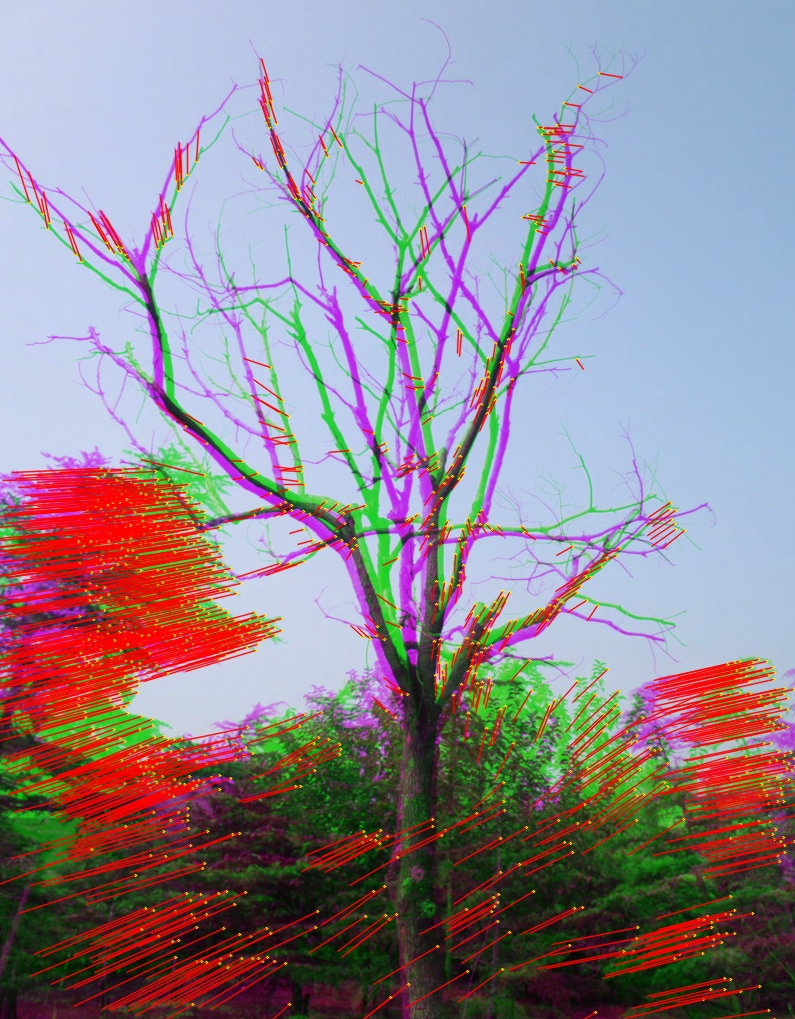
\includegraphics[height=10cm]{new.png}}
	\caption{Traditional PyrLK and Improved PyrLK}
	\label{fig:pyrlk}
\end{figure}


\clearpage
Algorithm \ref{alg:pyrlk} gives the pseudo-code of the improved PyrLK optical flow method:\\
\begin{algorithm}[H]
	\caption{Improved PyrLK}
	\label{alg:pyrlk}
	\begin{algorithmic}[1]
		\Require Image $I$,$J$,Point $\mathbf{u}$ in Image $I$
		\Ensure Corresponding point $\mathbf{v}$ in Image $J$
		\State Build the pyramidial representation of Image $I$ and $J$: $\{I^L\}_{L=0,...,L_m}$和$\{J^L\}_{L=0,...,L_m}$
		\State Initialize pyramid guess : $g^{L_{m}}=(g_x^{L_m}, g_y^{L_m})=(0,0)$
		\For{$L=L_m$to 0 with step of -1}
		\State Position point $\mathbf{u^L}$ in image $I^L$: $\mathbf{u}^L=(u_x,u_y)=\mathbf{u}/2^L$
		\State Assume $\mathbf{a_1}=(a_{11},a_{12},a_{13})\quad \mathbf{a_2}=(a_{21},a_{22},a_{23})\quad 
				\mathbf{b}=(d_x^L, d_y^L, 1$
		\State Define Similarity:
				\[ \epsilon(\mathbf{d^L})=\epsilon(d_x,d_y)=\sum_{x=u_x-\omega_x}^{u_x+\omega_x}\sum_{y=u_y-\omega_y}
				^{u_y+\omega_y}(I(x,y) - J(x+\mathbf{a_1}\cdot \mathbf{b},y+\mathbf{a_2}\cdot \mathbf{b}))^2.\]
				\State Least Squares to work out $d^L$,which let $\epsilon $ reach its minimum
		\State Guess on layer L-1: $g^{L-1}=2(g^L+d^L)$
		\EndFor
		\State Final optical flow vector: $\mathbf{d}=\mathbf{g^0}+\mathbf{d^0}$
		\State $\mathbf{v}=\mathbf{u+d}$
		\If{BackwardTrack$(\mathbf{v})$ = true}
			\If{MedianFilter$(\mathbf{v})$ = true}
				\State \Return $\mathbf{v}$
			\Else
				\State \Return NULL
			\EndIf
		\Else
			\State \Return NULL
		\EndIf
	\end{algorithmic}
\end{algorithm}

\section{本章小节}
\label{sec:conclusion}
本章首先介绍了光流法的由来,进而分析了LK光流法的思想和特点。然后对于基于图像金字塔的PyrLK光流法,它采用多分辨率图像层
来克服传统LK光流法无法捕捉图像中大块运动的缺陷。但是受缚于LK光流法的前提,该匹配算法只支持特征点的平移运动,由此带来很大
的束缚性。而且PyrLK光流法并没有对匹配的正确性进行验证,从而导致了很多错误的匹配对。基于这两方面的考虑,本章接着提出了支持
特征点旋转变换以及反向追踪的PyrLK光流法,这两个改进从根本上解决了PyrLK光流法的局限性,使PyrLK光流法的适用性和正确性都大大
的提升。本章的最后还给出了改进方法与传统方法的实验效果对比图。

\chapter{Tree Skeleton Extraction with 3D Voxel Flooding and Fitting}
\label{sec:sklextract}
After getting the point cloud model, under the consideration of lightweight processing,
we need to transfer the point cloud into logical structure. Using tree structure to represent
the tree is a natural idea, and the tree structure is a lightweight storage way compared to mesh.

This article 
在获取了精确的点云模型之后,出于后续轻量化的考虑,需要将模型的存储方式由
密集的点云转化为逻辑的父子结构。用树形的数据结构来表达现实的树结构,这是很
自然的想法,相对于面片结构,树形结构也是一种更为轻量化的存储方式。每个节点表示
树枝的起点,存储着该节点的空间位置,半径和该节点的父子枝信息以及兄弟信息。一个
节点和它的一个子节点形成一个空间线段,若干空间线段组成一条连续的树枝。

本文从树的生长规律入手,从根节点往子节点生长。生长的依据则为当前节点所在邻域
内的空间点云分布,节点邻域大小由步长来控制,步长会探索式地递增,直到达到了增长的阈值,
邻域大小才确定下来。然后从其点云分布拟合出各个分支的方向,从而生长出新的子节点,
并递归地生长下去直到点云的边界。

\section{三维体素模型}
前面三维重建步骤得到的结果是一个点云模型,该模型中的点数量庞大,不适于后续的
邻域搜索,因此我们需要对点云进行体素化处理。所谓体素化,就是将点云占据的空间
划分成一个个的小立方体,每一个立方体称之为一个体素。

在将点云模型转化为体素模型以后,对于点云的邻域搜索便转化为了对于空间临近体素的
搜索,体素的位置就反映了点集的位置,因此不用每次搜索都遍历整个点云,而是只用将
步长范围体素中的点集遍历即可。由于体素是我们处理的基本单位,所以体素的大小也
直接决定了体素模型的精度,因此,在确保非空体素的空间连续性和效率允许的基础上,
本文建议让体素尽可能的小,以保证模型的精度。将点云模型转换为体素模型的伪代码
在算法\ref{alg:voxel}中给出。图\ref{fig:voxel}形象地展示了将空间体素化以后树木的点云模型
在体素块中的分布情况。

\begin{figure}[H]
	\centering
	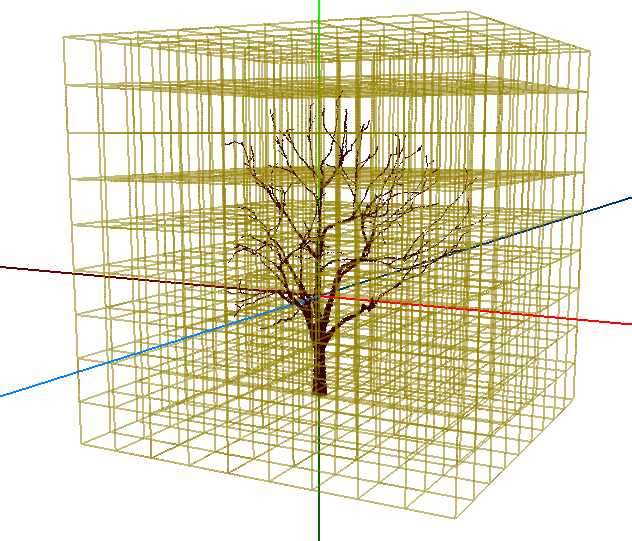
\includegraphics[height=8cm]{voxel.png}
	\caption{三维体素模型}
	\label{fig:voxel}
\end{figure}

\begin{algorithm}[H]
	\caption{点云模型体素化}
	\label{alg:voxel}
	\begin{algorithmic}[1] 
	\Require 点云模型$M$
	\Require 体素维度$d$
	\Ensure 三维体素数组$\mathbb{V}[1..d,1..d,1..d]$
	\State 初始化点云边界值$X_{max}=Y_{max}=Z_{max}=MIN\uline\quad FLOAT,X_{min}=Y_{min}=Z_{min}=MAX\uline\quad FLOAT$
	\ForAll{空间点$P(P_x,P_y,P_z) \in M$}
		\State $CheckBoundary(P)$
	\EndFor
\ForAll{空间点$P(P_x,P_y,P_z) \in M$}
\State $V_x = \frac{P_x-X_{min}}{X_{max}-X_{min}}\cdot d$
\State $V_y = \frac{P_y-Y_{min}}{Y_{max}-Y_{min}}\cdot d$
\State $V_z = \frac{P_z-Z_{min}}{Z_{max}-Z_{min}}\cdot d$
\State $\mathbb{V}[V_x, V_y, V_z] = \mathbb{V}[V_x, V_y, V_z] \bigcup \{P\} $
	\EndFor
\end{algorithmic}
\end{algorithm}

\section{三维体素泛洪确定邻域范围}
在确定了三维体素模型以后,便需要从根到叶,自底向上地对树的骨架结构进行生长。
生长的依据是已经得到的体素模型,将体素模型中点的分布作用于骨架的分支,便可以
张成骨架模型。

具体方法是将根节点置为当前节点,对其进行三维泛洪,首先对其相邻的26个体素进行泛洪,若
体素不为空,则将其加入邻域范围,若为空,则停止向该方向进行迭代。同时将加入邻域
范围的体素置为无效,表示其已经参与了泛洪,不再参与骨架的重建,这样不仅可以对算法
的结束有一个很好的约束条件,同时也可以减少重复处理的次数,加快算法的完成。然后进行下一次迭代,
对新加入的体素进行26方向的泛洪,并把有效的体素加入到邻域范围。接着比较两次迭代
体素增加的比例,如果低于设置的阈值,则停止迭代,当前的邻域范围即为三维泛洪得到
的当前节点的邻域范围。

图\ref{fig:3dfld}展示了三维体素泛洪确定邻域的步骤,三张图都延空间z轴正向投影到2D平面。
\ref{fig:3dfld}(a)为其初始状态,
即邻域范围为当前体素。其中橙色的区域表示邻域范围,蓝色的区域表示未探索区域,灰色区域
表示空的体素,而绿色区域表示已经在之前的枝干邻域。\ref{fig:3dfld}(b)表示体素泛洪经过
一次迭代以后的状态,因为体素泛洪只会对与当前邻域范围相邻的未探索区域(蓝色方块)进行扩展,
所以\ref{fig:3dfld}(a)只会向黄色箭头指向的体素进行扩展,从而得到\ref{fig:3dfld}(b)。在得到
新的邻域后,首先会计算所新增的点的数量与之前的数量的比值有没有低于阈值,如果低于阈值,则停止
邻域的扩张。最后将得到\ref{fig:3dfld}(c)中的邻域范围。

\begin{figure}[H]
	\centering
	\subfloat[初始状态(邻域范围为1个体素)]{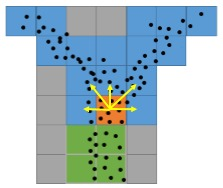
\includegraphics[height=3cm]{fld1.jpg}}\hspace{4em}
	\subfloat[第一次泛洪迭代(邻域范围为6个体素)]{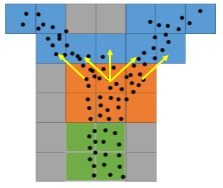
\includegraphics[height=3cm]{fld2.jpg}}\hspace{4em}
	\subfloat[第二次泛洪迭代(邻域范围为11个体素)]{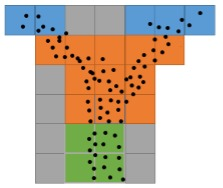
\includegraphics[height=3cm]{fld3.jpg}}
	\caption{体素泛洪示意图}
	\label{fig:3dfld}
\end{figure}

三维体素泛洪确定邻域范围算法的伪代码在算法\ref{alg:3dfld}中给出。
\begin{algorithm}[H] 
	\caption{三维体素泛洪确定邻域范围}
	\label{alg:3dfld}
	\begin{algorithmic}[1]
		\Require 当前体素$C$,三维体素数组$\mathbb{V}[1..d,1..d,1..d]$,
		泛洪方向数组$\mathbb{D}[1..26]$,邻域范围增长比例阈值$\lambda$
		%\Require 三维体素数组$\mathbb{V}[1..d,1..d,1..d]$
		%\Require 泛洪方向数组$\mathbb{D}[1..27]$
		%\Require 邻域范围增长比例阈值$\lambda$
		\Ensure	邻域范围内体素集合$\mathbb{S}$
		\State 初始化单次迭代新增体素集合$\mathbb{S'}$
		\State $\mathbb{S'}.AddVoxel($根节点所在体素$)$
		\ForAll{泛洪方向$Direction \in \mathbb{D}$}
			\State $NewIndex = C.Index + Direction$
			\State $NewVoxel = \mathbb{V}[NewIndex.x,NewIndex.y,NewIndex.z]$
			\If{$NewVoxel$非空$\bigcap NewVoxel$有效}
				\State $\mathbb{S'}.AddVoxel(NewVoxel)$
			\EndIf
		\EndFor
		\State 体素增长比例$\mu=\frac{\mathbb{S'}.VoxelCount}{\mathbb{S}.VoxelCount}$
		\If{$\mu > \lambda$}
			\ForAll{$voxel \in \mathbb{S'}$}
				\State 把$voxel$作为当前体素进行递归调用
			\EndFor
		\EndIf
		\State \Return $\mathbb{S}$
	\end{algorithmic}
\end{algorithm}

在进行三维泛洪的时候,可以编程实现26个方向迭代过程的并行化,以提高算法的效率。同时,值得注意的是,
为了将各个节点邻域范围探索的互相影响程度降到最低,本文将树木节点进行分级,即对每个节点,从根节点出发,
确定该节点是根节点的第几代子节点。本文对同一代的子节点进行并行化的邻域拓展,即对同一级的节点同时进行
泛洪,这样就可以避免一个子枝泛洪到另外一个子枝的邻域区域的错误。

\section{通过最小二乘法线性拟合确定分支方向}
\label{subsec:leastsquares}
当得到邻域范围以后,便得到了邻域内体素在基于当前节点26个方向上的密度分布,而
每个体素内又包含着若干的点,因此等于是得到了在当前节点邻域内的点云分布情况。
接下来的工作就是怎样从各个方向的点云的分布情况抽取出核心的骨架。本文应用线性
拟合的方法来从密集的点中抽取出一条直线,作为该部分的骨架方向。

该方法首先要剔除掉那些点云密度很小的方向,以免每个节点都朝各个方向长出一些
细碎的枝条。因为这些细碎的枝条就算在此步中不剔除,到后续的轻量化的时候也不容许
它们的存在。

然后对于剩下的若干方向$d_1,d_2...d_k$,每个方向都对应着树木的一个骨架。在处理
某个方向$d_i$时,将其包含的体素中的所有点抽取出来,得到一个密集的点集$S_i$。
然后采用待定方程的办法,设直线方程为:
\begin{equation}
	\mathbf{x} = \mathbf{x_0} + \mathbf{d}t,\quad(t \in [0,\infty))
\end{equation}

其中$\mathbf{x_0}$是当前节点的坐标,$\mathbf{d}$是待拟合的直线方向。我们假设
点集$S_i$中的点$P_1,P_2,...P_m$都在直线上,则可以得到以下方程组:\\

\begin{equation} \label{eq:line}
	\left\{ 
		\begin{array}{lll}
			a_{11}d_x+a_{12}d_y+a_{13}d_z & = & b1\\
			a_{21}d_x+a_{22}d_y+a_{23}d_z & = & b2\\
			... & & \\
			a_{n1}d_x+a_{n2}d_y+a_{n3}d_z & = & bn
		\end{array}
	\right.
\end{equation}

其中具体数值未给出,注意这里的$n=3m$,因为每个点$P$可以提供三个方向的方程式。
在这个方程组中,令\\
\begin{displaymath}
	\mathbf{U}=
\left(
\begin{array}{ccc}
	a_{11} & a_{12} & a_{13}\\
	a_{21} & a_{22} & a_{23}\\
	... & ... & ...\\
	a_{n1} & a_{n2} & a_{n3}\\
\end{array}
\right)
,\quad
\mathbf{d}=
\left(
\begin{array}{c}
	d_x\\
	d_y\\
	d_z
\end{array}
\right)
,\quad
\mathbf{b}=
\left(
\begin{array}{c}
	b_1\\
	b_2\\
	...\\
	b_n
\end{array}
\right)
\end{displaymath}


在实践中,由于筛选方向上的点数较多且发散分布,由线性代数的理论知,$\mathbf{U}$是过约束的,
即$n>r$,其中$r$是矩阵$\mathbf{U}$的秩。这种情况下没有标准的解,只能找到使误差最小的向量$\mathbf{d}$,
误差定义为:\\
\begin{equation}
	E\xlongequal{def} \sum_{i=1}^n(\mathbf{d}t_i - \mathbf{x_i} + \mathbf{x_0})^2=|\mathbf{Ud}-\mathbf{b}|^2
\end{equation}

由于$E$正比于方程的均方误差,因此只要E达到最小值,那么点集相对于该直线的波动就最
小。换句话说,也就是该直线最好的模拟了该点集所表示的骨架。由线性代数的方法很容易
可以解得$\mathbf{d}=\mathbf{[(U^TU)^{-1}U^T]b}$。图\ref{fig:fitting}展示了由当前
节点(蓝色节点)分别向两个点云集合拟合出的两条直线(红色线段),这两条直线将被作为两个
分支的方向。从图中可以看出线性拟合的方法可以很好的估计出树木分枝的方向,从而准确的
恢复出树木的父子结构。

\begin{figure}[H]
	\centering
	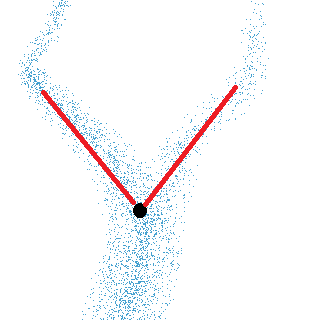
\includegraphics[height=5cm]{branch.png}
	\caption{线性拟合计算分支方向}
	\label{fig:fitting}
\end{figure}

算法\ref{alg:sklextract}给出了得到邻域信息后进行骨架方向抽取的伪代码,其中\textit{Least Squares Processing}表示运用最小二乘法进行
线性拟合。

\begin{algorithm}[H]
	\caption{基于邻域的骨架方向计算}
	\label{alg:sklextract}
	\begin{algorithmic}[1] 
		\Require 当前节点体素$V$
		\Require 骨架方向数组$\mathbb{D}[1..n]$
		\Ensure 当前节点子节点集合$\mathbb{S}$
		\ForAll{骨架方向$d\in D$}
			\State $NewChild\gets Least Squares Processing$
			\State $\mathbb{S}.AddChild(NewChild)$
		\EndFor
		\State \Return $\mathbb{S}$
	\end{algorithmic}
\end{algorithm}

\section{获取子枝长度和半径}
树木骨架的长度和半径对树木模型的真实感有着十分显著的贡献,所以尽可能准确的获得子枝的长度和
半径信息能够有助于重建出极具真实感的树木模型。对于树木枝干半径的获取方法有许多,
主要分为根据规则生成半径和从树木点云结构中获取半径两种方式。

对于基于规则来生成半径,最简单的方法是对树木半径进行线性地递减,即$r=cR$,其中
$r$为子枝半径,$R$是父枝半径,$c$为一个线性倍数,这个倍数可以固定,也可以进行
随机的扰动从而增进多样性。Leonardo da Vinci在经过大量观察后总结出了一种更符合自然规律
的树木父子枝直径的关系公式:$D^2=\sum_{i=1}^n{d_i^2}$,其中$D$为父枝直径,$d_i$为第
$i$个子枝的直径,$n$为子枝的数量。这个公式被广泛地用于树木枝干的半径模拟。

区别于基于规则的半径生成方法,本文为了进一步提升真实感,选择在进行子枝方向抽取的同时,
同样进行半径抽取的方法。注意,用该方法的前提是点云分布须均匀化,然而基于图像进行三维重建
得到的树木点云会呈现表皮化的现象,这是由于图片上的点都是树木的表皮点,所以在得到
三维点云后,是需要进行一些修复工作的,本文用随机点填充的方法对该点云模型进行了实心化
的修复。当点云分布满足均匀化时,在对某个骨架进行拟合之后,对于拟合出来的直线,来计算
所有参加拟合该直线的点到该直线的平均距离$D_{avg}$,然后就可以计算该骨架的半径$R=D_{avg}*2$。
由于点云分布均匀,所以半径显然就是平均距离的2倍。该算法的伪代码在算法\ref{alg:radius}中给出。\\

\begin{algorithm}[H]
	\caption{骨架半径抽取}
	\label{alg:radius}
	\begin{algorithmic}[1] 
		\Require 拟合出的当前子枝所在直线$L$
		\Require 当前子枝的点集$\mathbb{S}$
		\Ensure 当前子枝半径$R$
		\State 初始化点到直线距离之和$D_{sum}=0$
		\ForAll{空间点$P \in \mathbb{S}$}
		\State 点到直线距离$D_{sum}+=CalculateDistance(P, L)$
		\EndFor
		\State 平均距离$D_{avg}=D_{sum}/\mathbb{S}.Count$
		\State 子枝半径$R=D_{avg}*2$
		\State \Return $R$
	\end{algorithmic}
\end{algorithm}

图\ref{fig:radius}给出了三种半径求解方法的效果对比。\ref{fig:radius}(a)给出了线性衰减方法
的结果,该方法中子枝半径以父枝半径的线性倍衰减。\ref{fig:radius}(b)给出了前文提到的Leonardo
 da Vinci规则所生成的半径情况。\ref{fig:radius}(c)则采用本文中基于线性拟合直线,再计算所有点
 到该直线平均距离的方法。从三者的效果中可以看出,线性衰减容易出现部分枝条生长不自然的现象,究其
 原因,还是因为一个单一的绝对的线性系数无法适用于所有的枝条,它对于某些枝条会偏大,对于另外一些
 枝条会偏小。 Leonardo规则虽然给出的是一种父子枝之间的相对关系,从一定程度上解决了线性系数单一
 绝对而导致的问题,但是它生成的树木枝干会出现过于均与化,而没有捕捉到现实中树木各个局部的特征。
 本文的方法则由于其基于对所有点的实际恢复坐标进行统计,而更加注重树木的实际局部特征情况,
 其效果也是三者之中最好的。
 \begin{figure}[H]
	\centering
	\subfloat[样本图像]{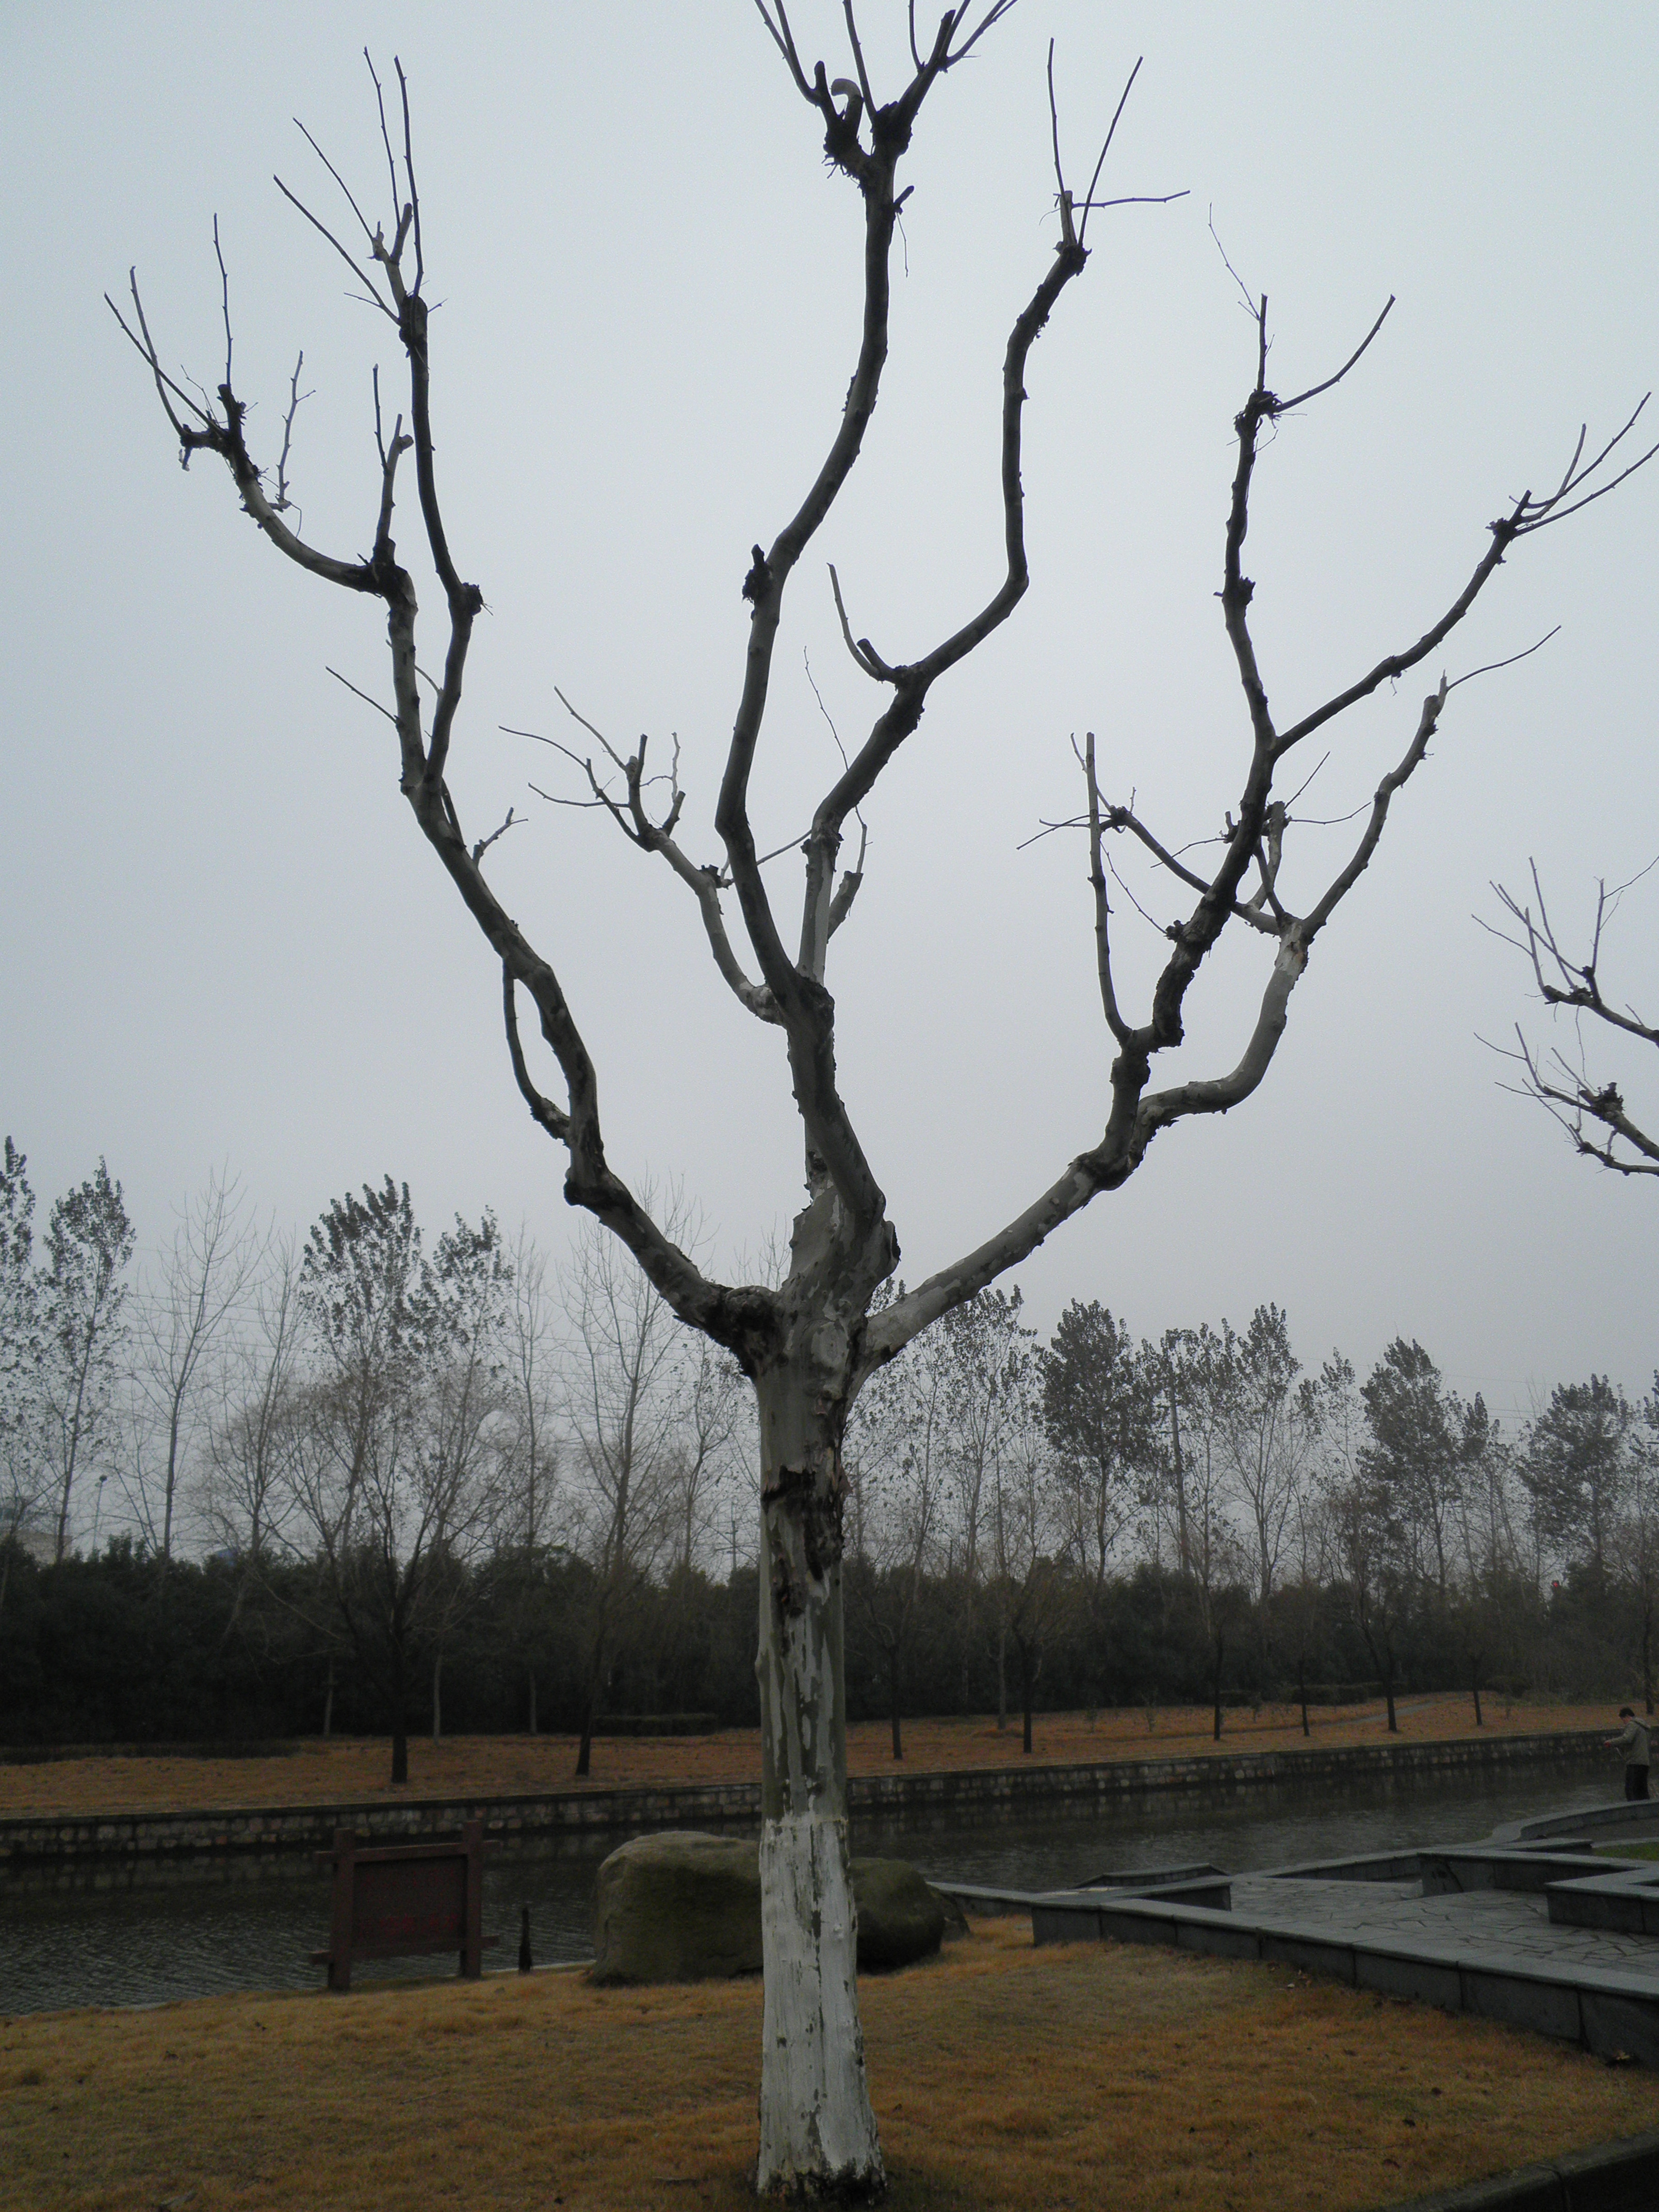
\includegraphics[height=6cm]{rsample.jpg}}\hspace{4em}
	\subfloat[线性衰减(线性衰减系数为0.6)]{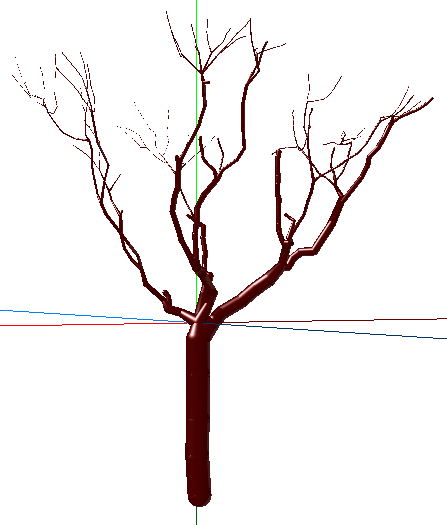
\includegraphics[height=6cm]{rlinear.png}}\hspace{4em}
	\subfloat[Leonardo规则生成($D^2=\sum_{i=1}^n{d_i^2}$)]{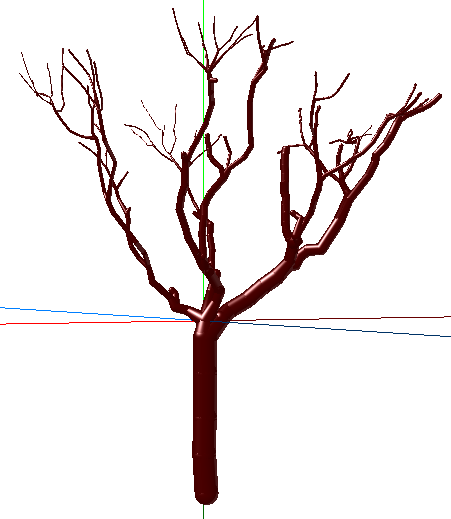
\includegraphics[height=6cm]{rsquare.png}}\hspace{4em}
	\subfloat[基于拟合的半径抽取]{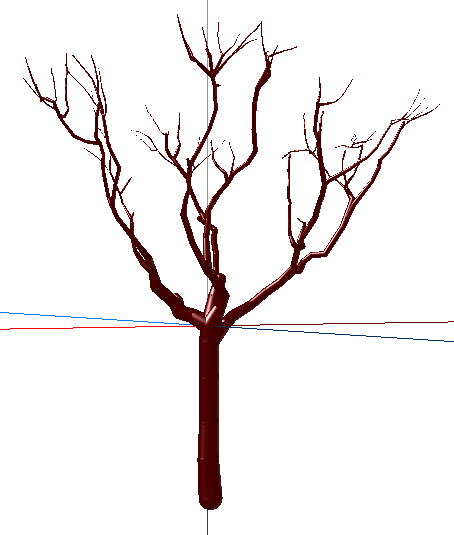
\includegraphics[height=6cm]{raffine.png}}\hspace{4em}
	\caption{三种计算半径方法效果对比}
	\label{fig:radius}
\end{figure}

对于骨架长度的估计,基于规则的生成则并不那么具有实践性,因为树木枝干的长度往往并不像半径那样
随着父子关系而递减。相反地,它地规则往往要复杂许多,而且并没有统一的规则。基于此考虑,本文并
没有对基于规则的长度估计进行实践,而是直接用与半径类似的方法,根据已拟合出的直线,试图从统计
的角度对其枝条长度做出合理的估计。一个直观而可行的方法,是将当前节点与所有该方向邻域的点的连线向量
投影到拟合出的直线方向向量上,这个投影的平均值的2倍,则可以估计为该方向子枝的长度。本文也给出了
子枝长度估计的伪代码,列在了算法\ref{alg:length}中。

\begin{algorithm}[H]
	\caption{子枝长度抽取}
	\label{alg:length}
	\begin{algorithmic}[1] 
		\Require 拟合出的当前子枝方向向量$L$,父节点$N$
		\Require 当前子枝的点集$\mathbb{S}$
		\Ensure 当前子枝长度$L$
		\State 初始化父节点到邻域点的向量投影长度之和$D_{sum}=0$
		\ForAll{空间点$P \in \mathbb{S}$}
		\State 父节点到$P$的向量$Dir=P$.Position-$N$.Position
		\State $Dir$在$L$上的投影距离$D_{sum}+=$CalculateProjectionLength$(Dir, L)$
		\EndFor
		\State 平均距离$D_{avg}=D_{sum}/\mathbb{S}.Count$
		\State 子枝长度$L=D_{avg}*2$
		\State \Return $L$
	\end{algorithmic}
\end{algorithm}

\section{本章小节}

三维体素泛洪是计算机图形学中二维像素泛洪的扩展,它将三维体素按洪水泛滥一般进行空间的扩展。本章利用三维体素泛洪实现了节点
对邻域的探索,该方法可以有效的避免枝条间的干扰,并提高邻域探索的效率。然后在该邻域的范围内对方向进行分割,将每个分割方向上
的点集根据最小二乘法进行拟合,得出该方向上骨架具体的直线方程。
然后根据点集内点到对应直线方程的距离大小,算出该骨架的半径大小,根据点集与当前节点连线在直线方向上的投影长度,来估算出枝干长度。
从而得到具有完整信息的骨架结构。

\include{data/chap06}
\include{data/chap07}
\include{data/chap08}
\include{data/chap09}

%%% 其它部分
\backmatter

\makeatother

% 致谢
\cleardoublepage

%%% Local Variables:
%%% mode: latex
%%% TeX-master: "../main"
%%% End:

\begin{ack}
  衷心感谢我的导师贾金原教授。在这一年的毕业设计过程中,贾老师严谨的治学作风、
  渊博的学术造诣以及悉心的指导给了我莫大的帮助和激励。不仅使我学到了如何高效率
  地工作,也让我学到了在治学方面所应该持有的执着又平淡的态度。使我从一个对
  计算机图形方面一无所知的门外汉,成为了深入其中并乐此不疲的钻研者。在论文完成
  之际,对贾老师表示最衷心的谢意。

  感谢同济大学软件学院在这本科四年中对我的培养,让我学会了做人,也让我对软件开发
  产生了浓厚的兴趣。感谢同济大学,你终将是我引以为傲的母校。在此希望学校和学院
  都越来越好。
  
  感谢实验室全体同学对我的帮助和支持。本课题承蒙国家自然科学基金资助,特此致谢。

  感谢\LaTeX{}的存在,虽然它没有所见即所得的直观,但却为我排版省下了不少时间,也
  使我的论文格式漂亮了很多。

\end{ack}


% 参考文献
\cleardoublepage
\bibliographystyle{tongjibib}
\bibliography{ref/refs}


% 附录
%\cleardoublepage
%\begin{appendix}
%%%% Local Variables:
%%% mode: latex
%%% TeX-master: "../main"
%%% End:

\chapter{外文资料原文}
\label{cha:engorg}
As one of the most widely used techniques in operations research, {\em
  mathematical programming} is defined as a means of maximizing a quantity known
as {\em objective function}, subject to a set of constraints represented by
equations and inequalities. Some known subtopics of mathematical programming are
linear programming, nonlinear programming, multiobjective programming, goal
programming, dynamic programming, and multilevel programming$^{[1]}$.

It is impossible to cover in a single chapter every concept of mathematical
programming. This chapter introduces only the basic concepts and techniques of
mathematical programming such that readers gain an understanding of them
throughout the book$^{[2,3]}$.


\section{Single-Objective Programming}
The general form of single-objective programming (SOP) is written
as follows,
\begin{equation}\tag*{(123)} % 如果附录中的公式不想让它出现在公式索引中,那就请
                             % 用 \tag*{xxxx}
\left\{\begin{array}{l}
\max \,\,f(x)\\[0.1 cm]
\mbox{subject to:} \\ [0.1 cm]
\qquad g_j(x)\le 0,\quad j=1,2,\cdots,p
\end{array}\right.
\end{equation}
which maximizes a real-valued function $f$ of
$x=(x_1,x_2,\cdots,x_n)$ subject to a set of constraints.

One of the outstanding contributions to mathematical programming was known as
the Kuhn-Tucker conditions\ref{eq:ktc}. In order to introduce them, let us give
some definitions. An inequality constraint $g_j(x)\le 0$ is said to be active at
a point $x^*$ if $g_j(x^*)=0$. A point $x^*$ satisfying $g_j(x^*)\le 0$ is said
to be regular if the gradient vectors $\nabla g_j(x)$ of all active constraints
are linearly independent.

%\newtheorem{mpdef}{Definition}[chapter]
%\begin{mpdef}
%In SOP, we call $x$ a decision vector, and
%$x_1,x_2,\cdots,x_n$ decision variables. The function
%$f$ is called the objective function. The set
%\begin{equation}\tag*{(456)} % 这里同理,其它不再一一指定。
%S=\left\{x\in\Re^n\bigm|g_j(x)\le 0,\,j=1,2,\cdots,p\right\}
%\end{equation}
%is called the feasible set. An element $x$ in $S$ is called a
%feasible solution.
%\end{mpdef}
%
%\newtheorem{mpdefop}[mpdef]{Definition}
%\begin{mpdefop}
%A feasible solution $x^*$ is called the optimal
%solution of SOP if and only if
%\begin{equation}
%f(x^*)\ge f(x)
%\end{equation}
%for any feasible solution $x$.
%\end{mpdefop}

Let $x^*$ be a regular point of the constraints of SOP and assume that all the
functions $f(x)$ and $g_j(x),j=1,2,\cdots,p$ are differentiable. If $x^*$ is a
local optimal solution, then there exist Lagrange multipliers
$\lambda_j,j=1,2,\cdots,p$ such that the following Kuhn-Tucker conditions hold,
\begin{equation}
\label{eq:ktc}
\left\{\begin{array}{l}
    \nabla f(x^*)-\sum\limits_{j=1}^p\lambda_j\nabla g_j(x^*)=0\\[0.3cm]
    \lambda_jg_j(x^*)=0,\quad j=1,2,\cdots,p\\[0.2cm]
    \lambda_j\ge 0,\quad j=1,2,\cdots,p.
\end{array}\right.
\end{equation}
If all the functions $f(x)$ and $g_j(x),j=1,2,\cdots,p$ are convex and
differentiable, and the point $x^*$ satisfies the Kuhn-Tucker conditions
(\ref{eq:ktc}), then it has been proved that the point $x^*$ is a global optimal
solution of SOP.

\subsection{Linear Programming}
\label{sec:lp}

If the functions $f(x),g_j(x),j=1,2,\cdots,p$ are all linear, then SOP is called
a {\em linear programming}.

The feasible set of linear is always convex. A point $x$ is called an extreme
point of convex set $S$ if $x\in S$ and $x$ cannot be expressed as a convex
combination of two points in $S$. It has been shown that the optimal solution to
linear programming corresponds to an extreme point of its feasible set provided
that the feasible set $S$ is bounded. This fact is the basis of the {\em simplex
  algorithm} which was developed by Dantzig as a very efficient method for
solving linear programming.
\begin{table}[ht]
\centering
  \centering
  \caption*{Table~1\hskip1em This is an example for manually numbered table, which
    would not appear in the list of tables}
  \label{tab:badtabular2}
  \begin{tabular}[c]{|c|m{0.8in}|c|c|c|c|c|}\hline
    \multicolumn{2}{|c|}{Network Topology} & \# of nodes &
    \multicolumn{3}{c|}{\# of clients} & Server \\\hline
    GT-ITM & Waxman Transit-Stub & 600 &
    \multirow{2}{2em}{2\%}&
    \multirow{2}{2em}{10\%}&
    \multirow{2}{2em}{50\%}&
    \multirow{2}{1.2in}{Max. Connectivity}\\\cline{1-3}
    \multicolumn{2}{|c|}{Inet-2.1} & 6000 & & & &\\\hline
    \multirow{2}{1in}{Xue} & Rui  & Ni &\multicolumn{4}{c|}{\multirow{2}*{\tongjithesis}}\\\cline{2-3}
    & \multicolumn{2}{c|}{ABCDEF} &\multicolumn{4}{c|}{} \\\hline
\end{tabular}
\end{table}

Roughly speaking, the simplex algorithm examines only the extreme points of the
feasible set, rather than all feasible points. At first, the simplex algorithm
selects an extreme point as the initial point. The successive extreme point is
selected so as to improve the objective function value. The procedure is
repeated until no improvement in objective function value can be made. The last
extreme point is the optimal solution.

\subsection{Nonlinear Programming}

If at least one of the functions $f(x),g_j(x),j=1,2,\cdots,p$ is nonlinear, then
SOP is called a {\em nonlinear programming}.

A large number of classical optimization methods have been developed to treat
special-structural nonlinear programming based on the mathematical theory
concerned with analyzing the structure of problems.
\begin{figure}[h]
  \centering
  
\includegraphics[clip]{tongji-lib-logo.jpg}
  \caption*{Figure~1\hskip1em This is an example for manually numbered figure,
    which would not appear in the list of figures}
  \label{tab:badfigure2}
\end{figure}

Now we consider a nonlinear programming which is confronted solely with
maximizing a real-valued function with domain $\Re^n$.  Whether derivatives are
available or not, the usual strategy is first to select a point in $\Re^n$ which
is thought to be the most likely place where the maximum exists. If there is no
information available on which to base such a selection, a point is chosen at
random. From this first point an attempt is made to construct a sequence of
points, each of which yields an improved objective function value over its
predecessor. The next point to be added to the sequence is chosen by analyzing
the behavior of the function at the previous points. This construction continues
until some termination criterion is met. Methods based upon this strategy are
called {\em ascent methods}, which can be classified as {\em direct methods},
{\em gradient methods}, and {\em Hessian methods} according to the information
about the behavior of objective function $f$. Direct methods require only that
the function can be evaluated at each point. Gradient methods require the
evaluation of first derivatives of $f$. Hessian methods require the evaluation
of second derivatives. In fact, there is no superior method for all
problems. The efficiency of a method is very much dependent upon the objective
function.

\subsection{Integer Programming}

{\em Integer programming} is a special mathematical programming in which all of
the variables are assumed to be only integer values. When there are not only
integer variables but also conventional continuous variables, we call it {\em
  mixed integer programming}. If all the variables are assumed either 0 or 1,
then the problem is termed a {\em zero-one programming}. Although integer
programming can be solved by an {\em exhaustive enumeration} theoretically, it
is impractical to solve realistically sized integer programming problems. The
most successful algorithm so far found to solve integer programming is called
the {\em branch-and-bound enumeration} developed by Balas (1965) and Dakin
(1965). The other technique to integer programming is the {\em cutting plane
  method} developed by Gomory (1959).

\hfill\textit{Uncertain Programming\/}\quad(\textsl{BaoDing Liu, 2006.2})

\section*{References}
\noindent{\itshape NOTE: these references are only for demonstration, they are
  not real citations in the original text.}

\begin{enumerate}[{$[$}1{$]$}]
\item Donald E. Knuth. The \TeX book. Addison-Wesley, 1984. ISBN: 0-201-13448-9
\item Paul W. Abrahams, Karl Berry and Kathryn A. Hargreaves. \TeX\ for the
  Impatient. Addison-Wesley, 1990. ISBN: 0-201-51375-7
\item David Salomon. The advanced \TeX book.  New York : Springer, 1995. ISBN:0-387-94556-3
\end{enumerate}

\chapter{外文资料的调研阅读报告或书面翻译}
\section{单目标规划}
北冥有鱼,其名为鲲。鲲之大,不知其几千里也。化而为鸟,其名为鹏。鹏之背,不知其几
千里也。怒而飞,其翼若垂天之云。是鸟也,海运则将徙于南冥。南冥者,天池也。
\begin{equation}\tag*{(123)}
 p(y|\mathbf{x}) = \frac{p(\mathbf{x},y)}{p(\mathbf{x})}=
\frac{p(\mathbf{x}|y)p(y)}{p(\mathbf{x})}
\end{equation}

吾生也有涯,而知也无涯。以有涯随无涯,殆已!已而为知者,殆而已矣!为善无近名,为
恶无近刑,缘督以为经,可以保身,可以全生,可以养亲,可以尽年。

\subsection{线性规划}
庖丁为文惠君解牛,手之所触,肩之所倚,足之所履,膝之所倚,砉然响然,奏刀騞然,莫
不中音,合于桑林之舞,乃中经首之会。
\begin{table}[ht]
\centering
  \centering
  \caption*{表~1\hskip1em 这是手动编号但不出现在索引中的一个表格例子}
  \label{tab:badtabular3}
  \begin{tabular}[c]{|c|m{0.8in}|c|c|c|c|c|}\hline
    \multicolumn{2}{|c|}{Network Topology} & \# of nodes &
    \multicolumn{3}{c|}{\# of clients} & Server \\\hline
    GT-ITM & Waxman Transit-Stub & 600 &
    \multirow{2}{2em}{2\%}&
    \multirow{2}{2em}{10\%}&
    \multirow{2}{2em}{50\%}&
    \multirow{2}{1.2in}{Max. Connectivity}\\\cline{1-3}
    \multicolumn{2}{|c|}{Inet-2.1} & 6000 & & & &\\\hline
    \multirow{2}{1in}{Xue} & Rui  & Ni &\multicolumn{4}{c|}{\multirow{2}*{\tongjithesis}}\\\cline{2-3}
    & \multicolumn{2}{c|}{ABCDEF} &\multicolumn{4}{c|}{} \\\hline
\end{tabular}
\end{table}

文惠君曰:“嘻,善哉!技盖至此乎?”庖丁释刀对曰:“臣之所好者道也,进乎技矣。始臣之
解牛之时,所见无非全牛者;三年之后,未尝见全牛也;方今之时,臣以神遇而不以目视,
官知止而神欲行。依乎天理,批大郤,导大窾,因其固然。技经肯綮之未尝,而况大坬乎!
良庖岁更刀,割也;族庖月更刀,折也;今臣之刀十九年矣,所解数千牛矣,而刀刃若新发
于硎。彼节者有间而刀刃者无厚,以无厚入有间,恢恢乎其于游刃必有余地矣。是以十九年
而刀刃若新发于硎。虽然,每至于族,吾见其难为,怵然为戒,视为止,行为迟,动刀甚微,
謋然已解,如土委地。提刀而立,为之而四顾,为之踌躇满志,善刀而藏之。”

文惠君曰:“善哉!吾闻庖丁之言,得养生焉。”


\subsection{非线性规划}
孔子与柳下季为友,柳下季之弟名曰盗跖。盗跖从卒九千人,横行天下,侵暴诸侯。穴室枢
户,驱人牛马,取人妇女。贪得忘亲,不顾父母兄弟,不祭先祖。所过之邑,大国守城,小
国入保,万民苦之。孔子谓柳下季曰:“夫为人父者,必能诏其子;为人兄者,必能教其弟。
若父不能诏其子,兄不能教其弟,则无贵父子兄弟之亲矣。今先生,世之才士也,弟为盗
跖,为天下害,而弗能教也,丘窃为先生羞之。丘请为先生往说之。”
\begin{figure}[h]
  \centering
  
\includegraphics{hello}
  \caption*{图~1\hskip1em 这是手动编号但不出现索引中的图片的例子}
  \label{tab:badfigure3}
\end{figure}

柳下季曰:“先生言为人父者必能诏其子,为人兄者必能教其弟,若子不听父之诏,弟不受
兄之教,虽今先生之辩,将奈之何哉?且跖之为人也,心如涌泉,意如飘风,强足以距敌,
辩足以饰非。顺其心则喜,逆其心则怒,易辱人以言。先生必无往。”

孔子不听,颜回为驭,子贡为右,往见盗跖。

\subsection{整数规划}
盗跖乃方休卒徒大山之阳,脍人肝而餔之。孔子下车而前,见谒者曰:“鲁人孔丘,闻将军
高义,敬再拜谒者。”谒者入通。盗跖闻之大怒,目如明星,发上指冠,曰:“此夫鲁国之
巧伪人孔丘非邪?为我告之:尔作言造语,妄称文、武,冠枝木之冠,带死牛之胁,多辞缪
说,不耕而食,不织而衣,摇唇鼓舌,擅生是非,以迷天下之主,使天下学士不反其本,妄
作孝弟,而侥幸于封侯富贵者也。子之罪大极重,疾走归!不然,我将以子肝益昼餔之膳。”


\chapter{其它附录}
其它附录的内容可以放到这里,当然如果你愿意,可以把这部分也放到独立的文件中,然后
将其\verb|\input| 到主文件中。
\section{测试附录}

%\end{appendix}

% 个人简历
%\cleardoublepage
%\begin{resume}

  \resumeitem{个人简历}

  xxxx 年 xx 月 xx 日出生于 xx 省 xx 县。
  
  xxxx 年 9 月考入 xx 大学 xx 系 xx 专业,xxxx 年 7 月本科毕业并获得 xx 学士学位。
  
  xxxx 年 9 月免试进入 xx 大学 xx 系攻读 xx 学位至今。

  \resumeitem{发表的学术论文} % 发表的和录用的合在一起

  \begin{enumerate}[{[}1{]}]
  \item Yang Y, Ren T L, Zhang L T, et al. Miniature microphone with silicon-
    based ferroelectric thin films. Integrated Ferroelectrics, 2003,
    52:229-235. (SCI 收录, 检索号:758FZ.)
  \item 杨轶, 张宁欣, 任天令, 等. 硅基铁电微声学器件中薄膜残余应力的研究. 中国机
    械工程, 2005, 16(14):1289-1291. (EI 收录, 检索号:0534931 2907.)
  \item 杨轶, 张宁欣, 任天令, 等. 集成铁电器件中的关键工艺研究. 仪器仪表学报,
    2003, 24(S4):192-193. (EI 源刊.)
  \item Yang Y, Ren T L, Zhu Y P, et al. PMUTs for handwriting recognition. In
    press. (已被 Integrated Ferroelectrics 录用. SCI 源刊.)
  \item Wu X M, Yang Y, Cai J, et al. Measurements of ferroelectric MEMS
    microphones. Integrated Ferroelectrics, 2005, 69:417-429. (SCI 收录, 检索号
    :896KM.)
  \item 贾泽, 杨轶, 陈兢, 等. 用于压电和电容微麦克风的体硅腐蚀相关研究. 压电与声
    光, 2006, 28(1):117-119. (EI 收录, 检索号:06129773469.)
  \item 伍晓明, 杨轶, 张宁欣, 等. 基于MEMS技术的集成铁电硅微麦克风. 中国集成电路, 
    2003, 53:59-61.
  \end{enumerate}

  \resumeitem{研究成果} % 有就写,没有就删除
  \begin{enumerate}[{[}1{]}]
  \item 任天令, 杨轶, 朱一平, 等. 硅基铁电微声学传感器畴极化区域控制和电极连接的
    方法: 中国, CN1602118A. (中国专利公开号.)
  \item Ren T L, Yang Y, Zhu Y P, et al. Piezoelectric micro acoustic sensor
    based on ferroelectric materials: USA, No.11/215, 102. (美国发明专利申请号.)
  \end{enumerate}
\end{resume}


\end{document}
